\documentclass[11pt]{article}
\usepackage{coling2016}
\usepackage{times}
\usepackage{url}
\usepackage{wrapfig}
\usepackage{graphicx}
\graphicspath{ {images/} }
%\bibliographystyle{acl}
%\bibliography{coling2016}

\title{Learning to Solve Arithmetic Word Problems using Sentence Simplification}

\author{First Author \\
  Affiliation / Address line 1 \\
  Affiliation / Address line 2 \\
  Affiliation / Address line 3 \\
  {\tt email@domain} \\\And
  Second Author \\
  Affiliation / Address line 1 \\
  Affiliation / Address line 2 \\
  Affiliation / Address line 3 \\
  {\tt email@domain} \\}
  
\begin{document}
\maketitle
\begin{abstract}
  This paper presents a sentence simplification approach to learning to solve arithmetic word problems. The approach performs a thorough analysis of each sentence in the given word problem to map each sentence to a simplified syntactic pattern. The syntactic pattern is generated by parsing the sentence using a dependency parser and encapsulates all the relevant information in a sentence including the subject, verb and object with its quantity as shown in Figure 1. The pattern is then used as a feature alongside other features as described in the Features section to classify the operator of the object given in the sentence. The classifier is trained on a small dataset of sentences and their operators and is not manually annotated. An equation is generated using similar information from multiple sentences in a given word problem.

  Using this approach the system learns to classify the operator with 70\% and is able to solve 70\% of the problems in the public dataset released by ~\cite{Hosseini:14} and can be found online\footnote{Dataset used is available at \url{https://www.cs.washington.edu/nlp/arithmetic}.}. The system overcomes some of the parsing issues encountered in attempt to solve word problems before and needs some improvement around the relational errors.
\end{abstract}
 
\section{Introduction}
\label{Intro}
Mathematical word problems are generally a sequence of actions by a subject on an object. The challenge in solving mathematical word problems is to extract information from a sentence accurately. Converting the extracted information to an equation is a trivial part. The complexities in extracting information increases when the sentence refers to an entity encountered in the previous sentences or some other related entities such as dollars and money.\newline

\begin{figure}[h]
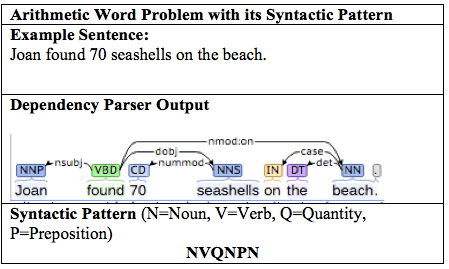
\includegraphics[width=0.6\textwidth]{Figure1}
\centering
\caption{\label{fig:Figure1}Example sentence of a word problem and its syntactic pattern.}
\end{figure}

When taking word problems into consideration, Algebra may be a challenging part from a child's point of view but the semantics of a sentence such as understanding of the syntax, extensive knowledge, coreference resolution and extracting information from individual sentences and combine that information effectively to produce a result.\newline

Our system needs to parse the sentences in a word problem well to fetch useful information. This information needs to be used collectively in an effective way to generate an equation. Solving the equation if generated correctly is a trivial part. Figure 1 shows an example of how a sentence from a word problem is simplified to a syntactic pattern. This paper approaches the problem of solving arithmetic word problems by mapping individual sentences in a word problem to a syntactic pattern. Based on the syntactic pattern each sentence is simplified till it represents minified information which consists of a subject, verb, object with its quantity and preposition if there exists one. This simplified sentence is then classified to an operator and the object with its quantity is added to the equation with the classified operator.\newline

Each simplified sentence is classified to one of four operators as described in Table ?. Our system learns this classifier based on the training data in section ?.

\section{Our Method}
\label{method}

In this section we describe how our system maps individual sentences of an arithmetic word problem to a syntactic pattern based on which it is further simplified and is assigned an operator by the classifier. There are several steps involved in this process and are described below:\newline

\subsection{Run Dependency Parser on Each Sentence}
The first step on a raw word problem text is to split it into multiple sentences and run dependency parser on each sentence. Based on the dependency parser output the sentence is mapped to a syntactic pattern as described in Figure 1. The further steps are based on the syntactic pattern of this sentence.

\subsection{Parse Commas in Each Sentence}
Commas play an important role in extracting the information from a sentence correctly. Hence, each sentence is looked for commas in it. After splitting the sentence on commas, the goal is to make each part a simplified sentence. For example: Joan has 20 seashells, 10 dollars and 20 cents in her bag will be simplified to 3 individual sentences: "Joan has 20 seashells in her bag. Joan has 10 dollars and 20 cents in her bag."

\subsection{Run Dependency Parser on Each Sentence}
Now that the sentences are simplified based on commas, they are again parsed through the dependency parser to get the simplified syntactic pattern which would further be used to simplify based on conjunctions.

\subsection{Parse Conjunctions in Each Sentence}
Conjunctions similar to commas help to simplify a sentence more concretely. The goal is again to have simplified sentences. For example: Joan has 10 dollars and 20 cents will be simplified to 2 individual sentences: "Joan has 10 dollars. Joan has 20 cents."

\subsection{Run Dependency Parser on Each Sentence}
The sentences are simplified at the most granular level and we run dependency parser on each of the simplified sentences. The syntactic pattern of each simplified sentence is used as a feature to classify this sentence to one of the four operators. There are some other features based on this syntactic pattern which are described in the Features section.

\subsection{Classification of the Feature Vector}
Based on the syntactic pattern of each simplified sentences, features are extracted from the pattern as described in the Features section. Based on the operator to which the sentence is classified, useful information from the sentence is merged into an equation for the word problem as a whole. 

\subsection{Using Quantified Noun in the Equation}
Based on the information extracted and the operator to which the sentence is classified, an equation is created or modified either by adding quantified nouns to the equation with its operator or an unknown quantity which needs to be calculated. For Example: The equation based on the extracted information for "Joan has 20 dollars. She gave 10 dollars to his friend. How many dollars does she have now?" will be +20 - 10 = ?.

\begin{thebibliography}{}
  
  \bibitem[\protect\citename{Hosseini \bgroup et al\egroup}2014]{Hosseini:14}
  Mohammad Javed Hosseini, Hannaneh Hajishirzi, Oren Etzioni and Nate Kushman.
  \newblock 2014.
  \newblock {\em In Proceedings of the EMNLP}
  
\end{thebibliography}

\end{document}